\chapter{Introduction}

  In today's society, people tend to spend much time on their mobile devices. Mobile devices are not just tool for communication, but also an essential tool for everyday tasks like doing our work, reading mail, pay our bills, and keeping up with our social life. Our whole life is contained in one device. When such a small device is so central to our daily lives, it makes it vulnerable.

  Passwords are human-chosen secrets that are connected to you as a person. When the password are created you might create a password that is an association to something you know or recognize; passwords are more than just words and numbers. Because of the shortcomings with text-based passwords \cite{UnixPasswords}, there is an increased interest in graphical passwords. The interest in graphical passwords started by the assumption that pictures are easier to remember and more secure than words and numbers \cite{DeAngeli}. Google's Android platform released the functionality for the Android Unlock Pattern in 2008. Since its release, there have been much discussion of its security, but few researchers have conducted scientific research on the Android Unlock Pattern. The problem is not just the theoretical password space, but the password space in practice.

  The motivation for this thesis started by observing the shortcomings with graphical passwords. Password reuse is one of the known password habits among users because the human limitation to remembering text-based password. Some users also make simple or meaningful password that are easier to remember, making their passwords vulnerable to attacks. Graphical passwords look like a promising alternative to text-based passwords, as it supports users to remember and make more complex passwords, offering better usability and higher security. As mobile devices play a significant role in our everyday life, it makes it interesting target device. Security on mobile devices has changed during the past years. The history of locking mechanisms was often a solution solely to prevent accidental use, while current mobile phones require protection in order to secure the potentially vast amount of private data that we keep on our smartphones. The situation of our rapid use of mobile phones, as well as it well-suited platform for graphical password, makes authentication on mobile devices an interesting field of study.

  In 2013, a research group conducted the first large-scale user study on the Android Unlock Patterns \cite{Uellenbeck}. The outcome of the research was an analysis of 2900 collected Android Unlock Patterns. They found bias in the pattern making process claiming that the scheme are less secure than its stated theoretical password space.

  This research aims to take the analysis of people's choice in Android Unlock Patterns a step further by including the human properties that may impact the user's choice in graphical passwords. This thesis is the first phase of my research and will continue in my master thesis in the following spring.

  \section{Research Questions}
    
    This thesis is the first phase of my research, and will be a supporting work for my master thesis. 

    {\bf $RQ1$: What is the status of current research on graphical passwords?} \\
    To answer this there will be conducted a literature review, and will give a overview of the research that is published in the field of graphical passwords. The goal is to get an overview, as well as find a gap in the research that this research can fill. 

    {\bf $RQ2$: What human properties may affect our choice of graphical passwords on mobile devices?}\\
    My motivation was to find if human properties impact users choice in graphical passwords. In order to find out, there need to be conducted a review on human properties that is found relevant to this research. 

  \section{Deliverables}

    The deliverables from this thesis are a literature review on graphical passwords to get an overview of published research, and provide a conceptual framework for the rest of the thesis. A literature review is providing the information needed to decide on the main research hypothesis for my master thesis, and the aim is to fill the gap in research on graphical passwords on mobile devices.

  As well as a literature review, there will be delivered a research design that will be used further in my master thesis. The research design is mainly a detailed description of the research strategy and data collection method. Research on passwords is not easy to conduct because of the nature of passwords. Passwords should remain a secret for the user, and as we have learned, we should not share our password due to security concerns. Research on text-based passwords is often based on leaked password on the web. When analyzing graphical passwords on mobile devices, there is no such data source available.
  
  The research design can provide insight into a new way of solving the problem of collecting user chosen passwords from mobile devices. This can provide knowledge for future research on graphical passwords on mobile devices.

  \section{Methods} \label{sec:method}

    \subsection{Research Process} \label{sec:methodresearchprocess}

    Throughout this thesis, the research process illustrated in figure~\ref{fig:researchProcess1} will be used as a starting point \cite{empiriske}. The research process is framework for researching information systems and computing. The model is not justed as a framework for this research project, but will be used as a model when designing the research that will be conducted in the following spring. The only part that is conducted in this thesis is the literature review for finding the research questions (hypothesis) to be used in my master thesis. The research strategy and data generation is described in section~\ref{chapter:researchDesign}.

      \begin{figure}[H]
        \centering
        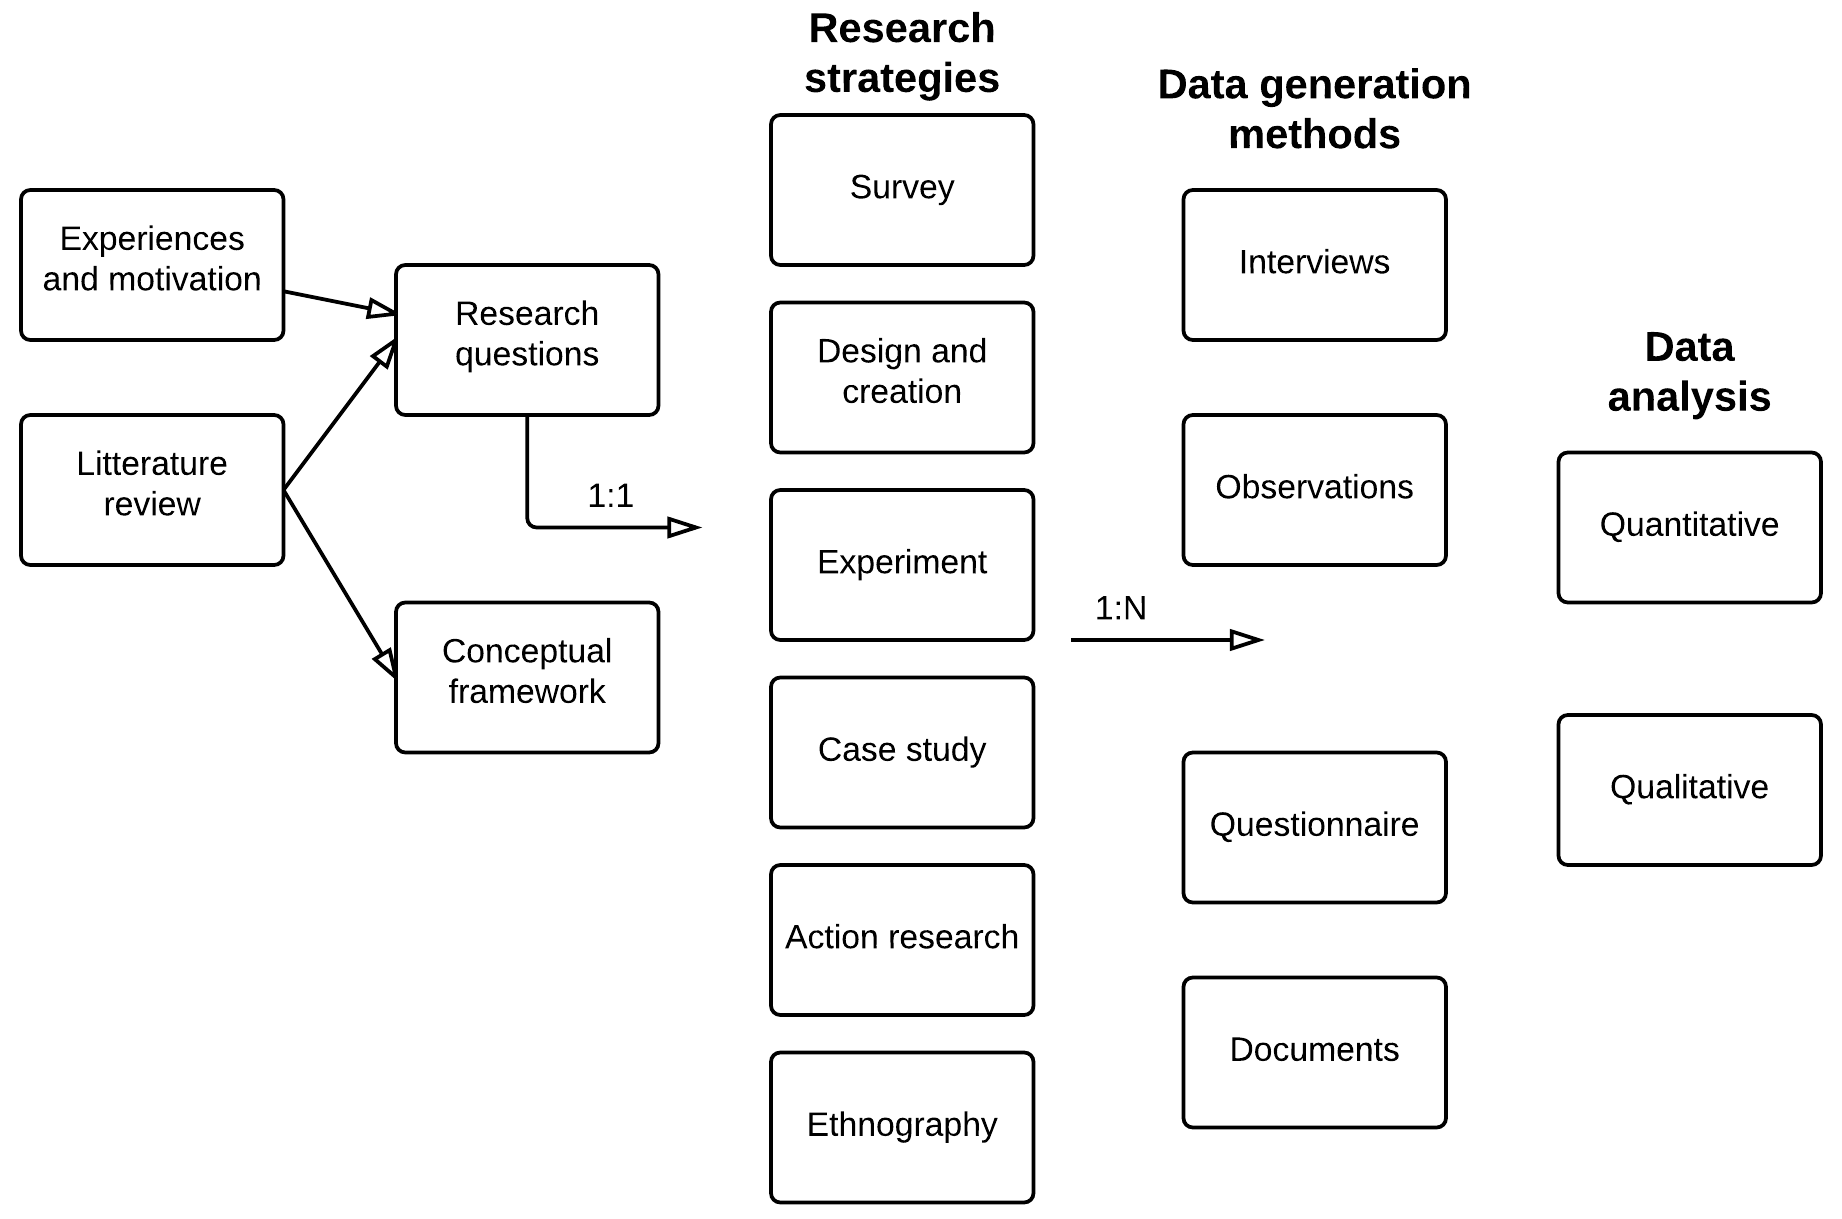
\includegraphics[scale=0.18]{pics/ResearchProcess.png}
        \caption[Research process]{Research Process \cite{empiriske}}
        \label{fig:researchProcess1}
      \end{figure}

    The Figure will appear later in the thesis in order to illustrate what parts of the research process that is being designed or conducted. In order to be able to understand the different parts of the research process, we will now provide an explanation of the different parts of the research process. 

    \todo{Beskrive alle delene research process i detalj}

    \subsection{Literature Review}\label{sec:methodliteraturereview}

    \subsection{Usability Testing} \label{sec:methodusabilitytesting}

  \section{Thesis structure}

    {\bf Chapter 2: Background Theory} presents the relevant background and theory that might improve the understanding of the information in the literature review. 

    {\bf Chapter 3: Literature Review} provides an overview of the current research on graphical passwords. 

    {\bf Chapter 4: Research Design} present the chosen research strategy and data collection method that will be used in my master thesis. 

    {\bf Chapter 5: Further Work} will be a discussion of the results from this thesis, and give a brief summary of the results. Further work will give a description of what will be conducted in the next phase of this research, my master thesis.  





